% ---------------------------------------------------------------
% Preamble
% ---------------------------------------------------------------
%\documentclass[a4paper,fleqn,longmktitle]{cas-sc}
\documentclass[a4paper,fleqn]{cas-dc}
%\documentclass[a4paper]{cas-dc}
%\documentclass[a4paper]{cas-sc}
% ---------------------------------------------------------------
% Make margins bigger to fit annotations. Use 1, 2 and 3. TO be removed later
%\paperwidth=\dimexpr \paperwidth + 6cm\relax
%\oddsidemargin=\dimexpr\oddsidemargin + 3cm\relax
%\evensidemargin=\dimexpr\evensidemargin + 3cm\relax
%\marginparwidth=\dimexpr \marginparwidth + 3cm\relax
% -------------------------------------------------------------------- 
% Packages
% --------------------------------------------------------------------
% Figure packages
\usepackage{graphicx,float}
\usepackage{adjustbox}
% Text, input, formatting, and language-related packages
\usepackage[T1]{fontenc}
\usepackage{subcaption}

\usepackage{csvsimple}

% TODO package
\usepackage[bordercolor=gray!20,backgroundcolor=blue!10,linecolor=black,textsize=footnotesize,textwidth=1in]{todonotes}
\setlength{\marginparwidth}{1in}
% \usepackage[utf8]{inputenc}
% \usepackage[nomath]{lmodern}

% Margin and formatting specifications
%\usepackage[authoryear]{natbib}
\usepackage[sort]{natbib}
\setcitestyle{square,numbers}

 %\bibliographystyle{cas-model2-names}

\usepackage{setspace}
\usepackage{subfiles} % Best loaded last in the preamble

% \usepackage[authoryear,longnamesfirst]{natbib}

% Math packages
\usepackage{amsmath, amsthm, amssymb, amsfonts, bm, nccmath, mathdots, mathtools, bigints, ulem}

\usepackage{tikz}
\usepackage{pgfplots}
\usetikzlibrary{shapes.geometric,angles,quotes,calc}

\usepackage{placeins}

\usepackage[final]{pdfpages}

% --------------------------------------------------------------------
% Packages Configurations
\usepackage{enumitem}
% --------------------------------------------------------------------
% (General) General configurations and fixes
\AtBeginDocument{\setlength{\FullWidth}{\textwidth}}	% Solves els-cas caption positioning issue
\setlength{\parindent}{20pt}
%\doublespacing
% --------------------------------------------------------------------
% Other Definitions
% --------------------------------------------------------------------
\graphicspath{{Figures/}}
% --------------------------------------------------------------------
% Environments
% --------------------------------------------------------------------
% ...

% --------------------------------------------------------------------
% Commands
% --------------------------------------------------------------------

% ==============================================================
% ========================== DOCUMENT ==========================
% ==============================================================
\begin{document} 
%  --------------------------------------------------------------------

% ===================================================
% METADATA
% ===================================================
\title[mode=title]{Sensitivity Analysis}                      
\shorttitle{Sensitivity Analysis}

\shortauthors{OS, PO}

\author[1]{Oliwer Sliczniuk}[orcid=0000-0003-2593-5956]
\ead{oliwer.sliczniuk@aalto.fi}
\cormark[1]
\credit{a}

\author[1]{Pekka Oinas}[orcid=0000-0002-0183-5558]
\credit{b}

%\author[1]{Francesco Corona}[orcid=0000-0002-3615-1359]
%\credit{c}

\address[1]{Aalto University, School of Chemical Engineering, Espoo, 02150, Finland}
%\address[2]{2}

\cortext[cor1]{Corresponding author}

% ===================================================
% ABSTRACT
% ===================================================
\begin{abstract}
This study aimed to investigate the supercritical extraction process of caraway oil from chamomile flowers. The distributed-parameter model describes the fluid-solid extraction process. The concept of quasi-one-dimensional flow is applied to reduce the number of spatial dimensions. The flow is assumed to be uniform across any cross-section, although the area available for the fluid phase can vary along the extractor. The physical properties of the solvent are estimated from the Peng-Robinson equation of state. A set of laboratory experiments was performed under multiple constant operating conditions: $30 - 40^\circ C$, $100 - 200$ bar, and $3.33-6.67 \times 10^{-5}$ kg/s. Sensitivity analyses play a crucial role in assessing the robustness of the findings or conclusions based on mathematical model. The local sensitivity analysis investigates the influence of infinitely small changes in the inlet temperature, pressure, and flow rate on the extraction yield.

\end{abstract}

\begin{keywords}
Supercritical extraction \sep Sensitivity analysis \sep Mathematical modelling
\end{keywords}

% ===================================================
% TITLE
% ===================================================
\maketitle

% ===================================================
% Section: Introduction
% ===================================================\section{Introduction}

\section{Introduction}
%\subfile{Sections/introduction}
\subfile{Sections/introduction_imp}

\subfile{Sections/Literature_Review}

%The study is structured as follows: Chapter \ref{CH: Thermodynamic} provides a general discussion on supercritical fluids to familiarize the reader with their properties. Chapter \ref{CH:Governing_equations_chapter} introduces the general balance equations. The balance equations are combined with the extraction kinetic equation to develop the process model in Chapter \ref{CH: Extraction_model}. The derivative-based local sensitivity analysis is presented in Chapter \ref{CH: Sensitivity_Analysis} and is then combined with the process model. Finally, the sensitivity plots are discussed in Chapters \ref{CH: Results} and \ref{CH: Conclusion}.

\section{Materials and methods} \label{CH: Materials and methods}

%\subsection{Supercritical fluids} \label{CH: Thermodynamic}
%\subfile{Sections/Thermo}
%\subfile{Sections/Thermo_imp}

%\clearpage
%\subfile{Sections/Materials_and_methods}

%\subsection{Governing equations} \label{CH:Governing_equations_chapter}
%\subfile{Sections/Gouverning_equation}

\subsection{Governing equations} \label{CH:Governing_equations_chapter}
Following the work of \citet{Anderson1995}, the governing equations for quasi-one-dimensional were derived. Quasi-one-dimensional flow refers to a fluid flow scenario assuming that flow properties are uniformly distributed across any given cross-section. This simplification is typically applied in situations where the flow channel's cross-sectional area changes, such as through irregular shapes or partial fillings of an extractor. According to this assumption, velocity and other flow properties change solely in the flow direction.

As discussed by \citet{Anderson2023}, all flows are compressible but some of them can be treated as incompressible when the Mach number is smaller than 0.3. This assumption leads to the incompressible condition: $\nabla \cdot u =0$, which is valid for constant density (strict incompressible) or varying density flow. The restraint allows for the removal of acoustic waves, and allows for large perturbations in density and/or temperature. In the 1-D case, the incompressibility condition becomes $\frac{du}{dz} = 0$, so the fluid velocity is constant.


%The governing equations based on the work of \citet{Anderson1995} for quasi-one-dimensional compressible flow in Cartesian coordinates are presented in Appendix \ref{CH: Gouverning equations}.

The set of quasi-one-dimensional governing equations in Cartesian coordinates is described by Equations \ref{EQ: CompressibleEuler_1} - \ref{EQ: CompressibleEuler_3}. %The formulation of these equations is elaborated upon in Appendix \ref{CH: Gouverning equations}, providing a mathematical foundation for analyzing flow dynamics under the assumed conditions.

{\footnotesize
	\begin{align}
		\label{EQ: CompressibleEuler_1}
		\cfrac{\partial \left( \rho_f A_f \right) }{\partial t} + \cfrac{\partial \left( \rho_f A_f v \right)}{\partial z} &= 0 \\
		\cfrac{\partial \left( \rho_f v A_f \right) }{\partial t} + \cfrac{\partial \left( \rho_f A_f v^2 \right)}{\partial z} &= -A_f \cfrac{\partial P}{\partial z} \label{EQ: CompressibleEuler_2} \\
		\cfrac{\partial \left( \rho_f e A_f \right) }{\partial t} + \cfrac{\partial \left( \rho_f A_f v e\right)}{\partial z} &= -P\cfrac{\left( A_f v \right)}{\partial z} + \cfrac{\partial}{\partial z} \left( k \cfrac{\partial T}{\partial z} \right)   
		\label{EQ: CompressibleEuler_3}
	\end{align}  
}

where $\rho_f$ is the density of the fluid, $A_f$ is the function which describe change of the cross-section, $v$ is the velocity, $P$ is the total pressure, $e$ is the internal energy of the fluid, $t$ is time and $z$ is the spacial direction.

\begin{comment}
	Based on governing equations, the small discontinuity (defined as $\delta$) in flow properties, shown in Figure \ref{fig: Discontinuity_slow_flow}, can be analysed. The analysis follows the work of \citet{Schreier1982}.
	
	\begin{figure}[!h]
		\centering
		\resizebox{0.95\columnwidth}{!}{%
			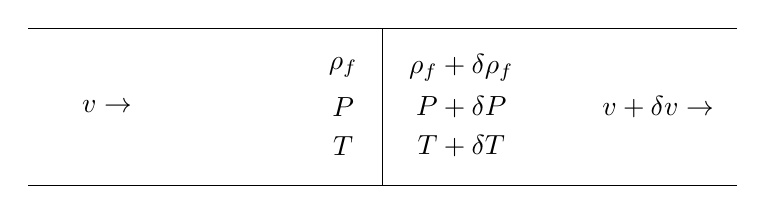
\begin{tikzpicture}[]
				\draw (0,2) -- (9,2);	% Top line
				\draw (0,0) -- (9,0); 	% Bottom line
				\draw (4.5,0) -- (4.5,2); 	% Bottom line
				\node at (4,1.5) {$\rho_f$};
				\node at (5.5,1.5) {$\rho_f+\delta\rho_f$};
				\node at (4,1.0) {$P$};
				\node at (5.5,1.0) {$P+\delta P$};
				\node at (4,0.5) {$T$};
				\node at (5.5,0.5) {$T+\delta T$};
				\node at (1,1.0) {$v \rightarrow$};
				\node at (8,1.0) {$v + \delta v \rightarrow$};
		\end{tikzpicture} }
		\caption{Small discontinuity in one-dimensional flow}
		\label{fig: Discontinuity_slow_flow}
	\end{figure} 
	
	The discontinuity is presumed to be at rest relative, and the balance equations become		
	
	{\footnotesize
		\begin{align*}
			&\rho_f \delta v + v \delta \rho_f + \delta \rho_f \delta v = 0 \\
			&\delta P = \delta v \delta \rho_f
		\end{align*}
	}
	
	These relations are equally valid if both regions are separated by a region of finite width rather than a discontinuity. 
	
	{\footnotesize
		\begin{equation*}
			\lim_{\rho_f v \rightarrow 0} \rho_f \delta v + v \delta \rho_f + \delta \rho_f \delta v = 0 / \delta \rho_f \rightarrow \cfrac{d v}{d \rho_f} = - \cfrac{v}{\rho_f}
		\end{equation*}
	}
	
	By combining the momentum equation with the above equation, we get
	
	{\footnotesize
		\begin{equation} \label{EQ: Pressure_Velocity}
			\cfrac{d v}{d \rho_f} = - \cfrac{d v}{dP} \cfrac{d P}{d \rho_f} = -\cfrac{1}{\rho v} \cfrac{dP}{d\rho_f} = -\cfrac{v}{\rho_f}
		\end{equation}
	}
	
	Suppose the flow is presumed to be isentropic, $dP/d\rho_f = c^2$, so $v^2=c^2$, where $c$ is the speed of sound. This can be interpreted as a small pressure wave propagating with the speed of sound relative to the flow. If the flow velocity is relatively low, all pressure changes are hydrodynamic (due to velocity motion) rather than thermodynamic, which leads to $\partial \rho_f / \partial P \approx 0$. The small changes in pressure due to flow velocity changes do not change the density. 
	
	The low Mach number condition leads to the incompressible condition: $\nabla \cdot u =0$, which is valid for constant density (strict incompressible) or varying density flow. The restraint allows for the removal of acoustic waves, but also allows for large perturbations in density and/or temperature. The assumption is that the flow remains within a Mach number limit (usually less than 0.3) for any solution using such a constraint to be valid. In the 1-D case, the incompressibility condition becomes $\frac{du}{dz} = 0$, so the fluid velocity is constant.
	
\end{comment}

\subsection{Extraction model} \label{CH: Extraction_model}
\subfile{Sections/Model}

%\newpage
%\section{Bayes theorem} \label{CH: Bayes}
%\subfile{Sections/Bayes_Theorem}
%\clearpage

\subsection{Sensitivity Analysis} \label{CH: Sensitivity_Analysis}
\subfile{Sections/Sensitivity_Analysis}

%\subsection{Experimental work}
%\subfile{Sections/Experiments}

\section{Results}
\subfile{Sections/Results_Sensitivity}

\section{Conclusions} \label{CH: Conclusion}

The sensitivity analysis is a tool to understand the parametric dependence in the dynamic behaviour of the analysed system. The presented formulation involves derivative-based local sensitivity analysis of the model solution with respect to selected parameters and controls. The sensitivity equations can be obtained in various ways, but the automatic differentiation technique was implemented to obtain the sensitivity equations in this work. By identifying which parameters are influential at each period of the simulation, local sensitivity analysis can yield valuable information for guiding the process modelling, the design of experiments or the model reduction. The local sensitivity analysis techniques consider the sensitivities at only a small region of parameter space, and the conclusions derived from such an analysis are limited to local conditions unless the discussed system is a linear model.

In this study, the local sensitivity analysis method was introduced to explore the dynamics of the supercritical extraction system, which consists of a set of partial differential equations. The sensitivity equations evaluate the influence of control variables such as flow rate, pressure, and inlet temperature on the state-space consisting of the concentration of the solute in solid and liquid phases, the fluid's enthalpy density, system pressure, and extraction yield. Every change in the control variables leads to a state-space change, eventually affecting the process performance. 

Similarities between Figures \ref{fig:Sensitivty_F_y}, \ref{fig:Sensitivty_P_y} and \ref{fig:Sensitivty_T_y} can observed, although the sources of disturbances are different. All the plots stay initially plat, and this is because the extraction kinetic is mainly controlled by the concentration gradient. The largest sensitivity deviations are observed in the second extraction phase, which is mainly controlled by the internal mass transfer. These deviations are strongly related to the fluid velocity and the correlations used to connect the extraction kinetic parameters. As correlations used in this work are linear functions of the fluid density( {\color{red} article 1}), Figures \ref{fig:Sensitivty_P_y} and \ref{fig:Sensitivty_T_y} are characterised by the opposite changes in the fluid density, which leads to the sensitivity plots with similar shape but opposite sign. In the third extraction phase, the concentration gradient and the internal diffusion coefficient decrease with the solute concentration in the solid phase( it is more difficult to extract the solute from the particle core than from the outer shell). It is important to note that the local-sensitivity methods obtain the discussed results, which can be obtained at different operating conditions.

This information can be utilized to identify which control variables influence the extraction yield the most. The controls with high sensitivities on the extraction can be used to investigate to find optimal operating conditions from an economic point of view.

% ===================================================
% Bibliography
% ===================================================
%% Loading bibliography style file
\clearpage
%\bibliographystyle{model1-num-names}
\bibliographystyle{unsrtnat}
\bibliography{mybibfile}

\clearpage \appendix \label{appendix}
\section{Appendix} 

\subsection{Thermodynamic}
\subfile{Sections/Qubic_EOS} \label{CH: EOS}

%\subsection{Governing equations}
%\subfile{Sections/Gouverning_equation_derivation}

%\subsection{Low Mach number expansion} \label{CH:Low_Mach_chapter}
%\subfile{Sections/Low_mach_number_expansion}
%\subfile{Sections/Low_mach_number_expansion_imp}

%\subsection{Bayes theorem} \label{CH: Bayes}
%\subfile{Sections/Bayes_Theorem}

\subsection{Cardano's Formula} \label{CH: Cardano}
\subfile{Sections/Cardano}

%\subsection{Initial and boundary conditions} \label{CH: IC_BC}
%\subfile{Sections/IC_BC}

%\subsection{Maximum Likelihood} \label{CH: ML}
%\subfile{Sections/Likelihood}

%\subsection{Solid density measurement} \label{CH: Solid_Density_Measurment}

%\begin{figure}[!h]
%	\centering 
%	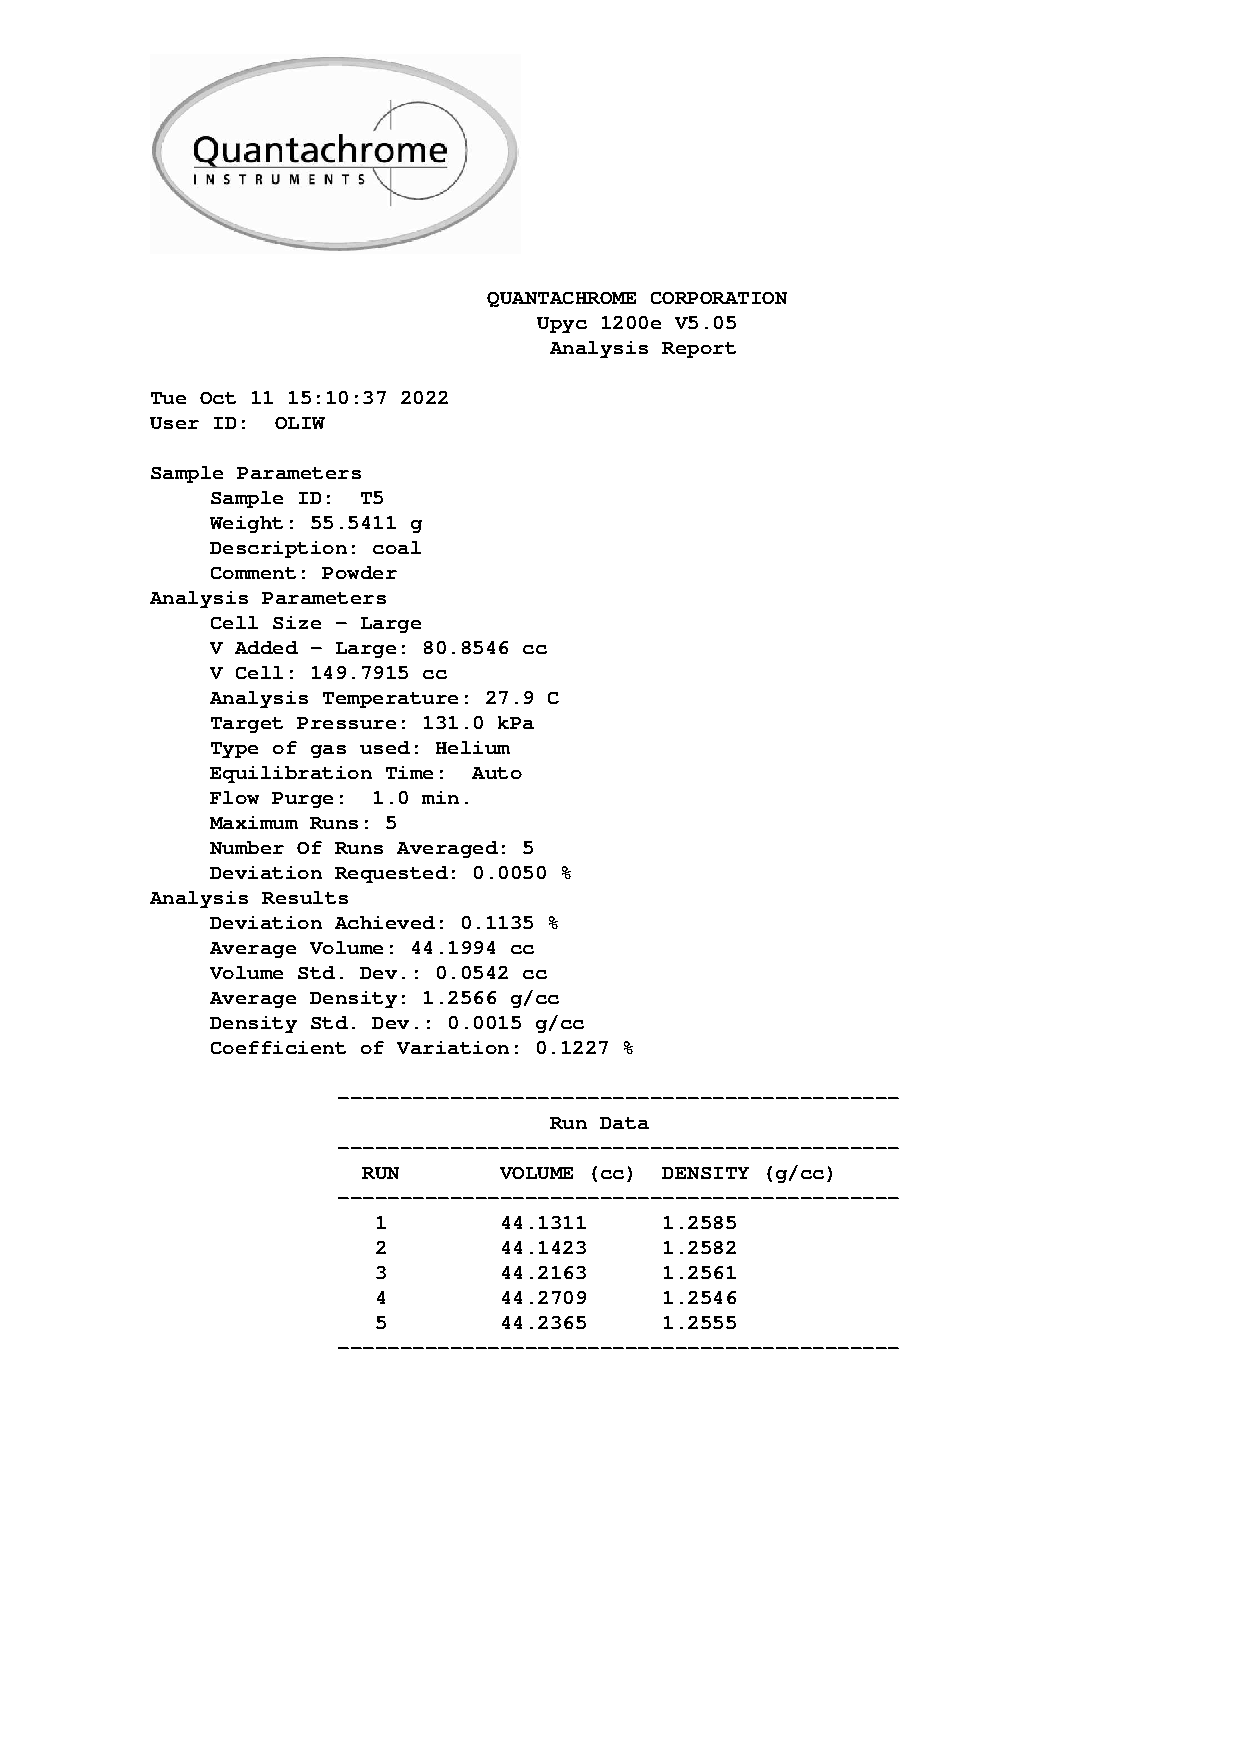
\includegraphics[trim=2cm 6cm 4cm 0cm, clip,width=\columnwidth]{Sections/ultraReportT5.pdf}
%	\caption{The result of solid density measurement}
%\end{figure}

%{\footnotesize
%	\begin{equation*}
%		\rho_s^{ave} = \frac{1.2585+1.2582+1.2561+1.2546+1.2555}{5} = 1.25658 [g/cc]
%	\end{equation*} }

%\subsection{Porosity Calculations} \label{CH: Porosity}
%\subfile{Sections/Porosity}

%\subsection{Concentration profiles} \label{CH: Profiles}
%\subfile{Sections/Profiles}

%\subsection{Solution of the parameter estimation starting from another initial guess} \label{CH: Profiles_2}
%\subfile{Sections/Parameter_estimation_solution_from_another_IG}

\end{document}